\section{Ziel}
\label{sec:Ziel}

Ziel des Versuches ist es die Grundlagen der Vakuumphysik zu erlernen. Dafür wird eine Evakuierungskurve für zwei verschiedene Pumptypen, einer Drehschieberpumpe
und einer Turbomolekularpumpe, durchgeführt. Es wird außerdem das effektive Saugvermögen beider Pumpen mithilfe einer Leckratenmessung bestimmt.

\section{Theorie}
\label{sec:Theorie}

\subsection{Theorie des Vakuum}
\label{subsec:vakuum}

(Nach \cite{EinfuehrungVakuum}) Als Vakuum wird der Zustand eines Gases bezeichnet, wenn der Druck innerhalb dieses Behälters unterhalb dem Druck außerhalb ist. Alternativ wird das Vakuum als Druckbereich unterhalb
$\SI{300}{\milli\bar}$ bezeichnet, dem geringstmöglichen Druck auf der Erdoberfläche (\cite{Vakuumtechnik}). Eine Möglichkeit verschiedene Bereiche von Vakuen zu beschreiben ist über die mittlere freie Weglänge $\bar l$, die die
Strecke beschreibt, bis ein Teilchen im Mittel auf ein anderes trifft. Sie ist definiert als
\begin{align}
    \bar l = \frac{k_B T}{\sqrt 2 \pi p d_m^2},
\end{align}
wobei $d_m$ der Moleküldurchmesser, $p$ der Druck, $k_B$ die Boltzmann-Konstante und $T$ die Temperatur ist.
Das Vakuum ist dabei in verschiedene Teilbereiche einzuordnen, die in Abhängigkeit vom Druck
und der mittleren freien Weglänge $\bar l$, in \autoref{tab:Vakuen} aufgetragen sind.

\begin{table}[H]
    \centering
    \caption{Druckbereiche in der Vakuumtechnik \cite{EinfuehrungVakuum}.}
    \label{tab:Vakuen}
    \begin{tabular}{c c c}
        \toprule
        Druckbereich & Druck / hPa &  mittlere freie Weglänge $\bar l$ / m\\
        \midrule
        Atmosphärendruck    & $1.013,25$    & $6,8\cdot10^{-8}$   \\
        Grobvakuum (GV)     & $300 - 1$     & $10^{-8}-10^{-4}$   \\
        Feinvakuum (FV)     & $1 - 10^{-3}$ & $10^{-4} - 10^{-1}$ \\
        Hochvakuum (HV)     & $10^{-3} - 10^{-8}$ & $10^{-1} - 10^{4}$ \\
        Ultrahochvakuum (UHV) & $10^{-8} - 10^{-11}$ & $10^{4} - 10^{7}$ \\
        Extrem hohes Vakuum (XHV) & $<10^{-11}$ & $<10^{-7}$ \\
        \bottomrule
    \end{tabular}
\end{table}

\noindent
Der Druck wird mithilfe der barometrischen Höhenformel als das Gewicht der über einer Fläche stehenden Luftsäule beschrieben,
\begin{align}
    \label{eqn:baroFormel1}
    p_h = p_0\cdot \exp\left({-\frac{\rho_o gh}{p_0}}\right).
\end{align}
Dabei ist $p_h$ der Druck bei der Höhe $h$, $p_0$ der Atmosphärendruck auf Meereshöhe (\SI{1013,25}{\hecto\pascal}), $g$ die Erdbeschleunigung und $\rho_0$ die Dichte der Luft
auf Meereshöhe bei $\SI{0}{\celsius}$  ($\SI{1,293}{\kilo\gram\per\meter\cubed}$).
Wird angenommen, das die Dichte der Luft, die Erdbeschleunigung und der Atmosphärendruck auf Meereshöhe konstant sind, folgt eine vereinfachte Darstellung der barometrischen
Höhenformel,
\begin{align}
    \label{eqn:baroFormel2}
    p_h = p_0\cdot\exp\left(-\frac{h}{\SI{8,005}{\meter}}\right).
\end{align}

\subsection{Das ideale Gas}
\label{subsec:idGas}

Das Modell des idealen Gases ist eine vereinfachende Beschreibung für reale Gase. Die idealen Gasteilchen sind dabei frei und üben keine Anziehungs- oder Abstoßungskräfte 
aufeinander aus. Es finden lediglich elastische Stöße zwischen der Wand des Behälters, in dem sich das Gas befindet, und zwischen den Teilchen selber statt. Die Teilchen selber
belegen dabei aber kein Volumen und können nicht rotieren oder vibrieren. Die kinetische Energie der Gasteilchen ist ausschließlich die translatorische Bewegung
im Raum. \newline
(Nach \cite{EinfuehrungVakuum}) Aus dem Boyle-Mariott'schen Gesetz $pV=const$ folgt, dass das Volumen einer Gasmenge bei konstanter Temperatur umgekehrt proportional zum Druck
ist. Gemeinsam mit dem Gay-Lussac'schen Gesetz $V=const\cdot T$, der Stoffmenge, der allgemeinen Gaskonstanten mit der Avogrado-Konstanten, die die Boltzmann-Konstante bilden,
folgt die allgemeine Gasgleichung,
\begin{align}
    \label{eqn:allgGasgl}
    pV=Nk_BT.
\end{align}
Dabei ist $p$ der Druck, $V$ das Volumen, der Teilchenzahl $N$ und $T$ die Temperatur.

\subsection{Strömungsarten}
\label{subsec:stroemungsarten}

Wenn von der Bewegung von flüssigen oder gasförmigen Teilchenmassen gesprochen wird, wird zwischen verschiedenen Arten der Bewegung unterschieden, den Strömungsarten. Das Verhältnis 
von mittlerer freier Weglänge $\bar l$ und dem Druchmesser $d$ des Strömungskanals wird zur Beschreibung von Strömungsarten verwendet und als Knudsenzahl bezeichnet,
\begin{align}
    Kn = \frac{\bar l}{d}.
\end{align}
Strömungen mit einer Knudsenzahl von $Kn < 0,01$ werden als viskose oder Kontinuumsströmung bezeichnet und sind im Grobvakuum vorzufinden. Ab einer Knudsenzahl von $Kn > 0,5$ wird 
von einer molekularen Strömung gesprochen und beschreibt Bewegungen im Hoch- und Ultrahochvakuum. Im Bereich 
$(0,01 < Kn < 0,05)$ befindet sich die als Knudsenströmung bezeichnete Strömung, die sich im Feinvakuum befindet. In \autoref{fig:stroemi} ist eine schematische Darstellung von verschiedenen Strömungsarten in Abhängigkeit der jeweiligen Knudsenzahl
eingezeichnet.
\begin{figure}[H]
    \centering
    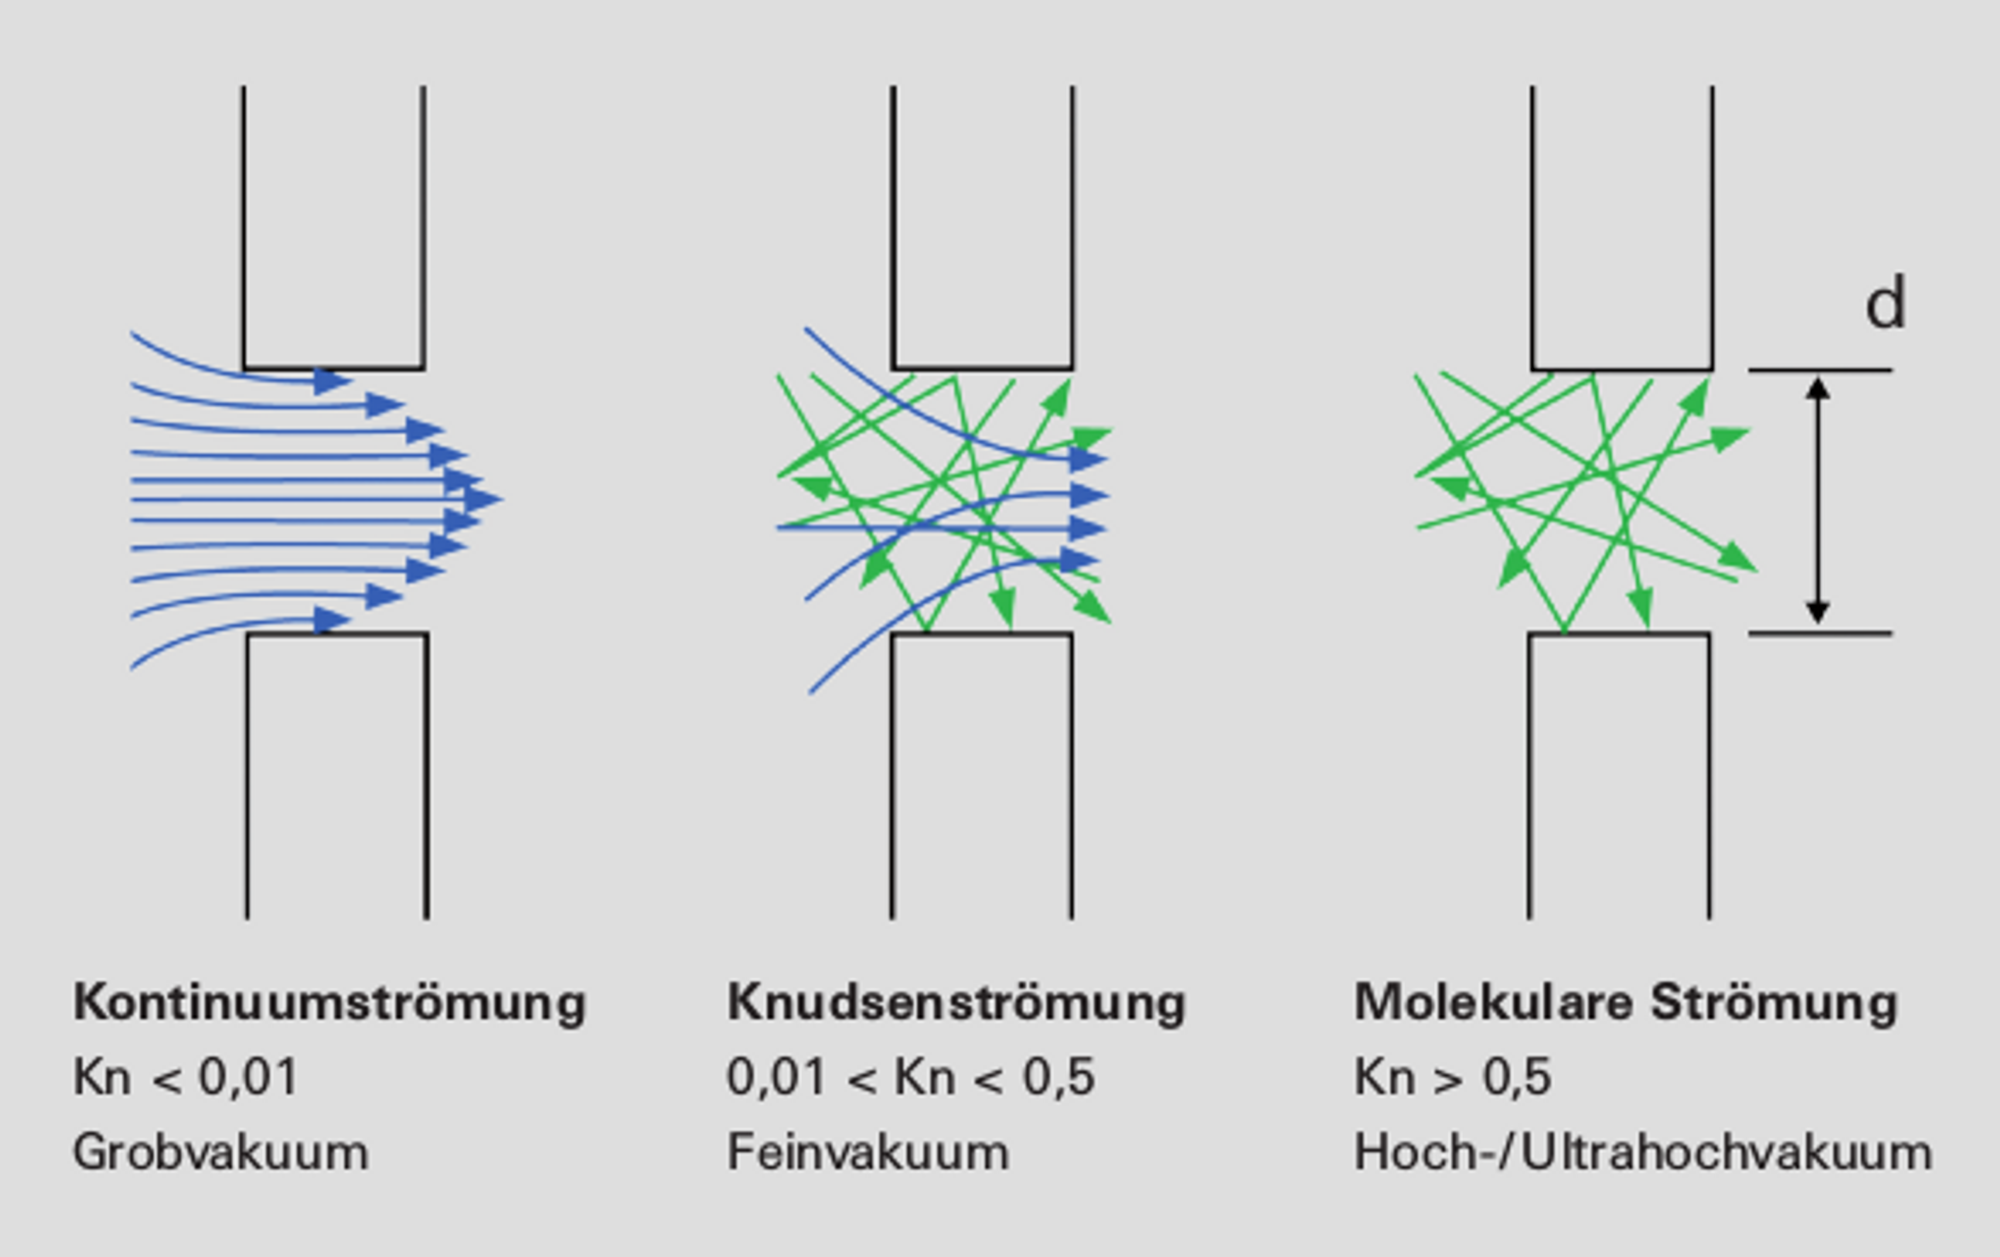
\includegraphics[width=0.7\textwidth]{data/stroemungen.png}
    \caption{Skizze der verschiedenen Strömungsarten in Abhängigkeit der Knudsenzahlen \cite{EinfuehrungVakuum}.}
    \label{fig:stroemi}
\end{figure}

\noindent
Bei viskosen Strömungen wird zusätzlich zwischen laminaren und turbulenten Strömungen unterschieden. Laminare Strömungen werden auch als Schichtströmungen bezeichnet, da die Gasteilchen immer in gleichen, parallelen Schichten
zueinander transportiert werden. Wenn die Strömungsgeschwindigkeit steigt, dann lösen sich die Schichten der Gasteilchen auf und die Teilchen sind vollkommen ungeordnet. Es wird von einer turbulenten Strömung gesprochen.
Die Grenze zwischen laminarer und turbulenter Strömung ist ein kontinuierlicher, der mathematisch durch die Reynoldszahl $Re$ beschrieben wird. Sie berechnet sich über die Dichte des Fluids $\rho$, die Strömungsgeschwindigkeit $\nu$,
die charakteristische Länge $l$ und die dynamische Viskosität $\eta$ über
\begin{align}
    Re= \frac{\rho\nu l}{\eta}.
\end{align}
Unter einer Reynoldszahl von $Re< 2.300$ wird von laminaren und ab $Re>4.000$ von turbulenten Strömungen gesprochen. In Vakuum kommen turbulente Strömungen nur beim Abpumpen des Atmosphärendrucks oder bei schnellem Belüften vor.
In \autoref{fig:lamiturbi} ist eine schematische Darstellung von turbulenter und laminarer Strömung in einem Kanal dargestellt.

\begin{figure}[H]
    \centering
    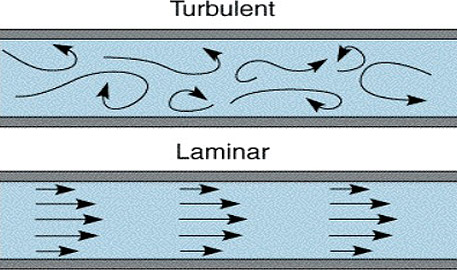
\includegraphics[width=0.7\textwidth]{data/LaminarTurbulent.jpeg}
    \caption{Laminare und turbulente Strömungen in einem Kanal \cite{LaminarTurbulent}.}
    \label{fig:lamiturbi}
\end{figure}

\subsection{Verunreinigungen}
\label{subsec:verunreinigungen}

In den zu vakuumierenden Behältern sind häufig Verunreinigungen. Das können Rückstände von der Produktion der Vakuumsysteme, Öle und Fette an Oberflächen, Schraubungen
und Dichtungen sein. Es können auch Stäube und Partikel zurückbleiben, die das System verunreinigen. Abscheidungen flüssiger oder fester Stoffe aus der Gaphase, die als Kondensationen
bezeichnet werden, setzen sich an den Behälterwänden ab. Die größte Verunreinigung ist dabei das kondensierter Wasserdampf aus der Umgebungsluft, welches sich an den Behälterwänden absetzt. 
Raumluft enthält in etwa $\SI{10}{\gram}$ Wasserdampf pro Kubikmeter, weshalb es sich an allen Oberflächen festsetzt. \newline
Verunreinigungen sind deshalb ein Problem, weil sie, auch wenn bereits der Großteil des Gases abgepumpt wurde, von den Wänden gelöst werden und somit der Druck nicht auf das gewünschte
Arbeitsniveau sinken kann.

\subsection{Saugvermögen und Saugleistung einer Vakuumpumpe}
\label{subsec:Saugleistung}

\noindent
Wird die allgemeine Gasgleichung (\ref{eqn:allgGasgl}) durch die Zeit $t$ dividiert, so folgt ein Gasstrom
\begin{align}
    q_{pV}=\frac{p\cdot V}{t} = \frac{mRT}{Mt}.
    \label{eqn:Gasstrom}
\end{align}

\noindent
Wird nun eine gleiche Temperatur angenommen, dann folgt ein konstant geförderter Massenstrom, der als pV-Durchfluss bezeichnet wird. Aus diesem folgt die Saugleistung einer Pumpe
\begin{align}
    q_{pV} = S\cdot P=\frac{\text dV}{\text dt}\cdot p,
\end{align}
die, dividiert durch den Eingangsdruck, das Saugvermögen ergibt,
\begin{align}
    S=\frac{\text dV}{\text dt}.
\end{align}

\noindent
Wird ein konstantes Saugvermögen angenommen, so kann durch das Ableiten der allgemeinen Gasgleichung (\ref{eqn:allgGasgl}) nach der Zeit $t$ die folgende Differentialgleichung aufgestellt werden
\begin{align}
    \dot pV=-pS,
\end{align}
dessen Lösung die Evakuierungskurve $p(t)$ ist, die den zeitlichen Verlauf des Druckes gemäß
\begin{align}
    p(t)=p_0\cdot\exp\left(-\frac{S}{V}\cdot t\right)
\end{align}
beschreibt.

\subsection{Leckrate}
\label{subsec:leckrate}

Neben offensichtlichen Lecks, wie undichte Flansche oder Schraubungen, können sogar aus Metallwänden kleine Gasströme entweichen. Solche Lecks werden als virtuelle Lecks bezeichnet.
Der Permeationsgasstrom $Q_{\text{Perm}}$, also der Strom eines Gases, der durch eine Barriere diffundiert, ist proportional zum Druckgradienten über die Wandstärke mit einer materialabhängigen Permeationskonstanten $k_{\text{Perm}}$,
\begin{align}
    \label{eqn:permeaStrom}
    Q_{\text{Perm}} = k_{\text{Perm}} A\cdot\frac{p_a}{d},
\end{align}
wobei $p_a$ der Druck außerhalb des Behälters, $A$ die Oberfläche des Behälters und $d$ die Wanddicke ist. Die Leckrate $Q_L$ ist nun der Strom des Gases, der durch die Undichtigkeiten in den Behälter strömt, ist folgendermaßen definiert
\begin{align}
    Q_L=\frac{\upDelta p V}{\upDelta t}.
\end{align}
Die Druckänderung während der Messzeit ist dabei mit $\upDelta p$ bezeichnet worden, $V$ ist das Volumen des Behälters und $\upDelta t$ die Messzeit.

\subsection{Drehschiebervakuumpumpe}
\label{subsec:Drehschieberpumpe}

(Nach Quelle \cite{Drehschiebervakuumpumpen}) Die Drehschiebervakuumpumpe ist eine ölüberlagert Rotationsverdrängerpumpe. Ein schematischer Aufbau mit Beschriftung der einzelnen Komponenten ist in \autoref{fig:drehschieberpumpe} dargestellt.

\begin{figure}[H]
    \centering
    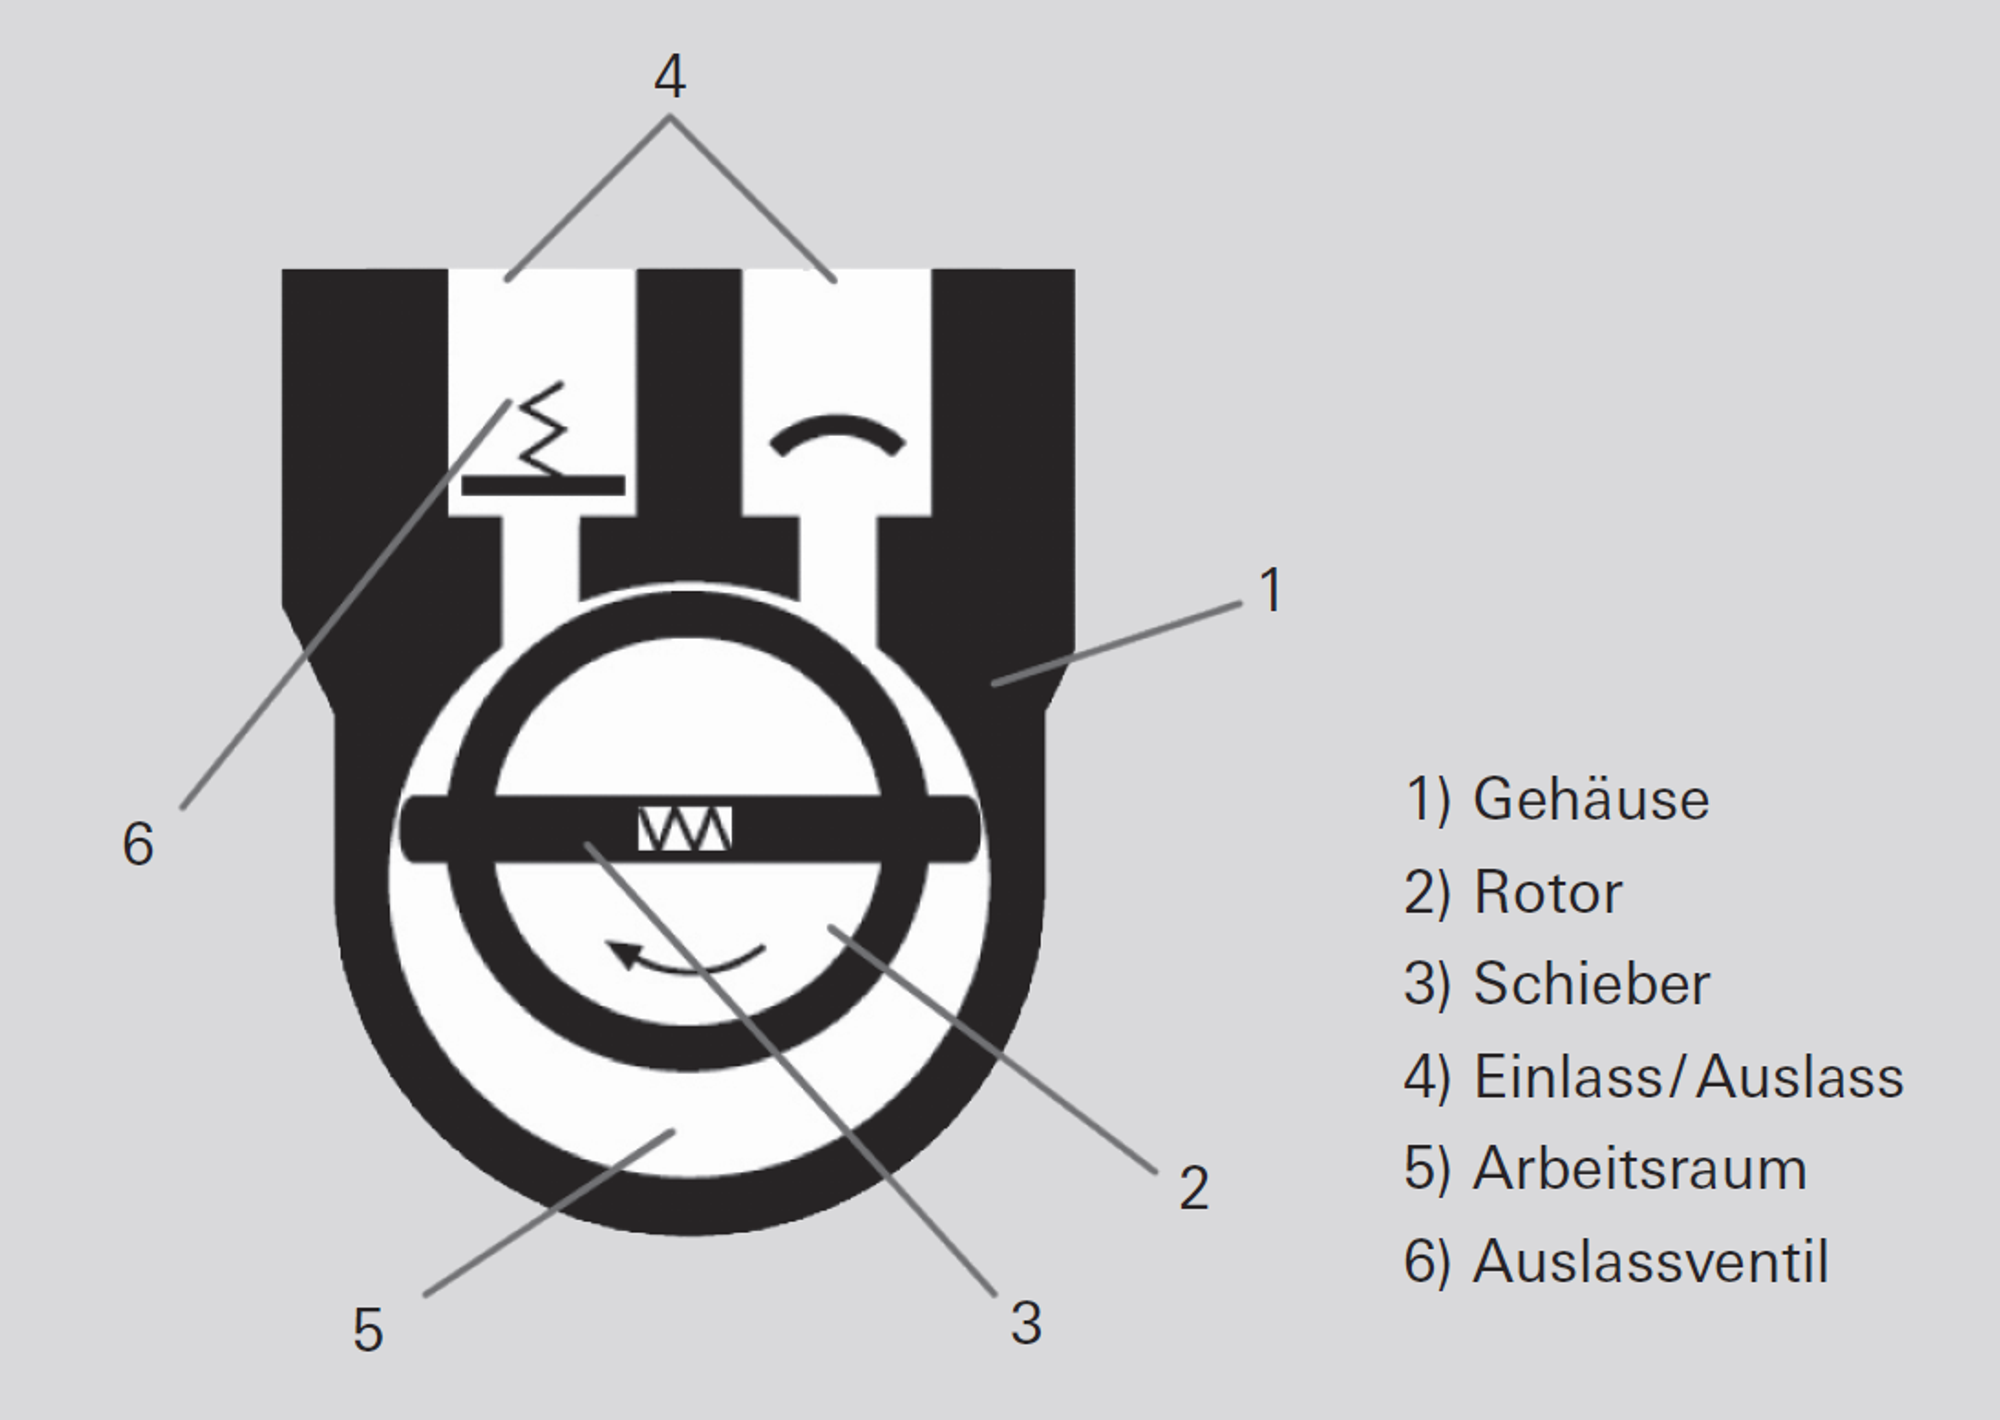
\includegraphics[width=0.7\textwidth]{data/drehschieberpumpe.png}
    \caption{Schematische Darstellung einer Drehschiebervakuumpumpe \cite{Drehschiebervakuumpumpen}.}
    \label{fig:drehschieberpumpe}
\end{figure}

\noindent
Der Rotor und der Schieber teilen den Arbeitsraum in zwei separate Räume mit variierbarem Volumen. Wenn sich der Rotor dreht, dann strömt Gas in den Schöpfraum, bis er durch den zweiten Schieber abgesperrt wird. Das eingeschlossene Gas wird dann so lange komprimiert, bis es durch den zweiten Schieber 
abgeschlossen wird und sich das Auslassventil gegen den Atmosphärendruck öffnet. Das Auslassventil ist ölüberlagert, wodurch beim Öffnen des Ventils eine kleine Menge Öl in den Schöpfraum dringt und den Schieber gleichzeitig gegen das Gehäuse abdichtet und schmiert.
Drehschiebervakuumpumpen werden in ein- oder zweistufigen Ausführungen eingebaut und auch als Vorpumpen verwendet.

\subsection{Turbomolekularpumpe}
\label{subsec:turbopumpe}

(Nach Quelle \cite{Turbomolekularpumpen}) Turbomolekularpumpen zählen zu der Kategorie der kinetischen Vakuumpumpen und ähneln im Aufbau einer Turbine. In einem Gehäuse rotiert ein mehrstufiger, turbinenartiger Rotor mit Schaufeln, die die Luft beschleunigen und somit ein Vakuum erzuegen. Durch die Lagerung der 
Rotoren mit zwei mit Schmierstoffen beschichteten Kugellagern müssen beide Lager vor der Vakuumseite angeordnet werden. Turbomolekularpumpen werden zum evakuieren großer Gefäße mit Drehschiebervakuumpumpen als Vorpumpen betrieben. Durch die hohe Rotationsfrequenz von $\SI{1350}{\hertz}$ ist es wichtig vor Betrieb einer Turbomolekularpumpe ein 
Vorvakuum zu erzeugen. Die zufälligen Kollisionen der Gasmoleküle werden dadurch unterdrückt und der Rotor wird nicht so leicht durch Reibung beschädigt. Turbopumpen funktionieren bei einem geringeren Ansaugdruck besser, als bei einem höheren, weshalb es auch für die Effizienz besser ist ein Vorvakuum zu erzeugen.
Ein typischer Verlauf des Saugvermögens in Abhängigkeit des Ansaugdruckes von Turbomolekularpumpen ist in \autoref{fig:SaugvermögenTurbo} abgebildet.
 
\begin{figure}[H]
    \centering
    \includegraphics[width=0.7\textwidth]{data/saugvermögenTurbo.png}
    \caption{Typischer Verlauf des Saugvermögens einer Turbomolekularpumpe in Abhängigkeit des Ansaugdruckes \cite{Turbomolekularpumpen}.}
    \label{fig:SaugvermögenTurbo}
\end{figure}

\subsection{Vakuummessgeräte}
\label{subsec:vakuummesser}

Im folgenden werden die im Versuch verwendeten Vakuummessgeräte nach Quelle \cite{Totaldruckmessung} beschrieben.

\subsubsection{Piezo-Vakuummeter}
\label{subsubsec:piezo}
(Nach \cite{Druckmessung}) Ein Piezo-Vakuummeter ist ein direktes, gasartunabhängiges Membran-Vakuummeter. Bei Membran-Vakuummetern wirkt auf eine Membran der Fläche $A$ der Druck $p$ und lenkt die Membran proportional zum Druck aus.
Im Falle eines Piezo-Vakuummeters wird der Druck durch piezo-resistive oder kapazitive Sensoren in ein elektrisches Signal umgewandelt, indem die Widerstandsänderung infolge der Membranauslenkung gemessen wird.
Ein schematischer Aufbau eines Piezo-Membranvakuummeters ist in \autoref{fig:piezo} eingezeichnet. Dabei wird der Druck des evakuierten Volumens mit $p$ und der Referenzdruck mit $p_0$ bezeichnet.

\begin{figure}[H]
    \centering
    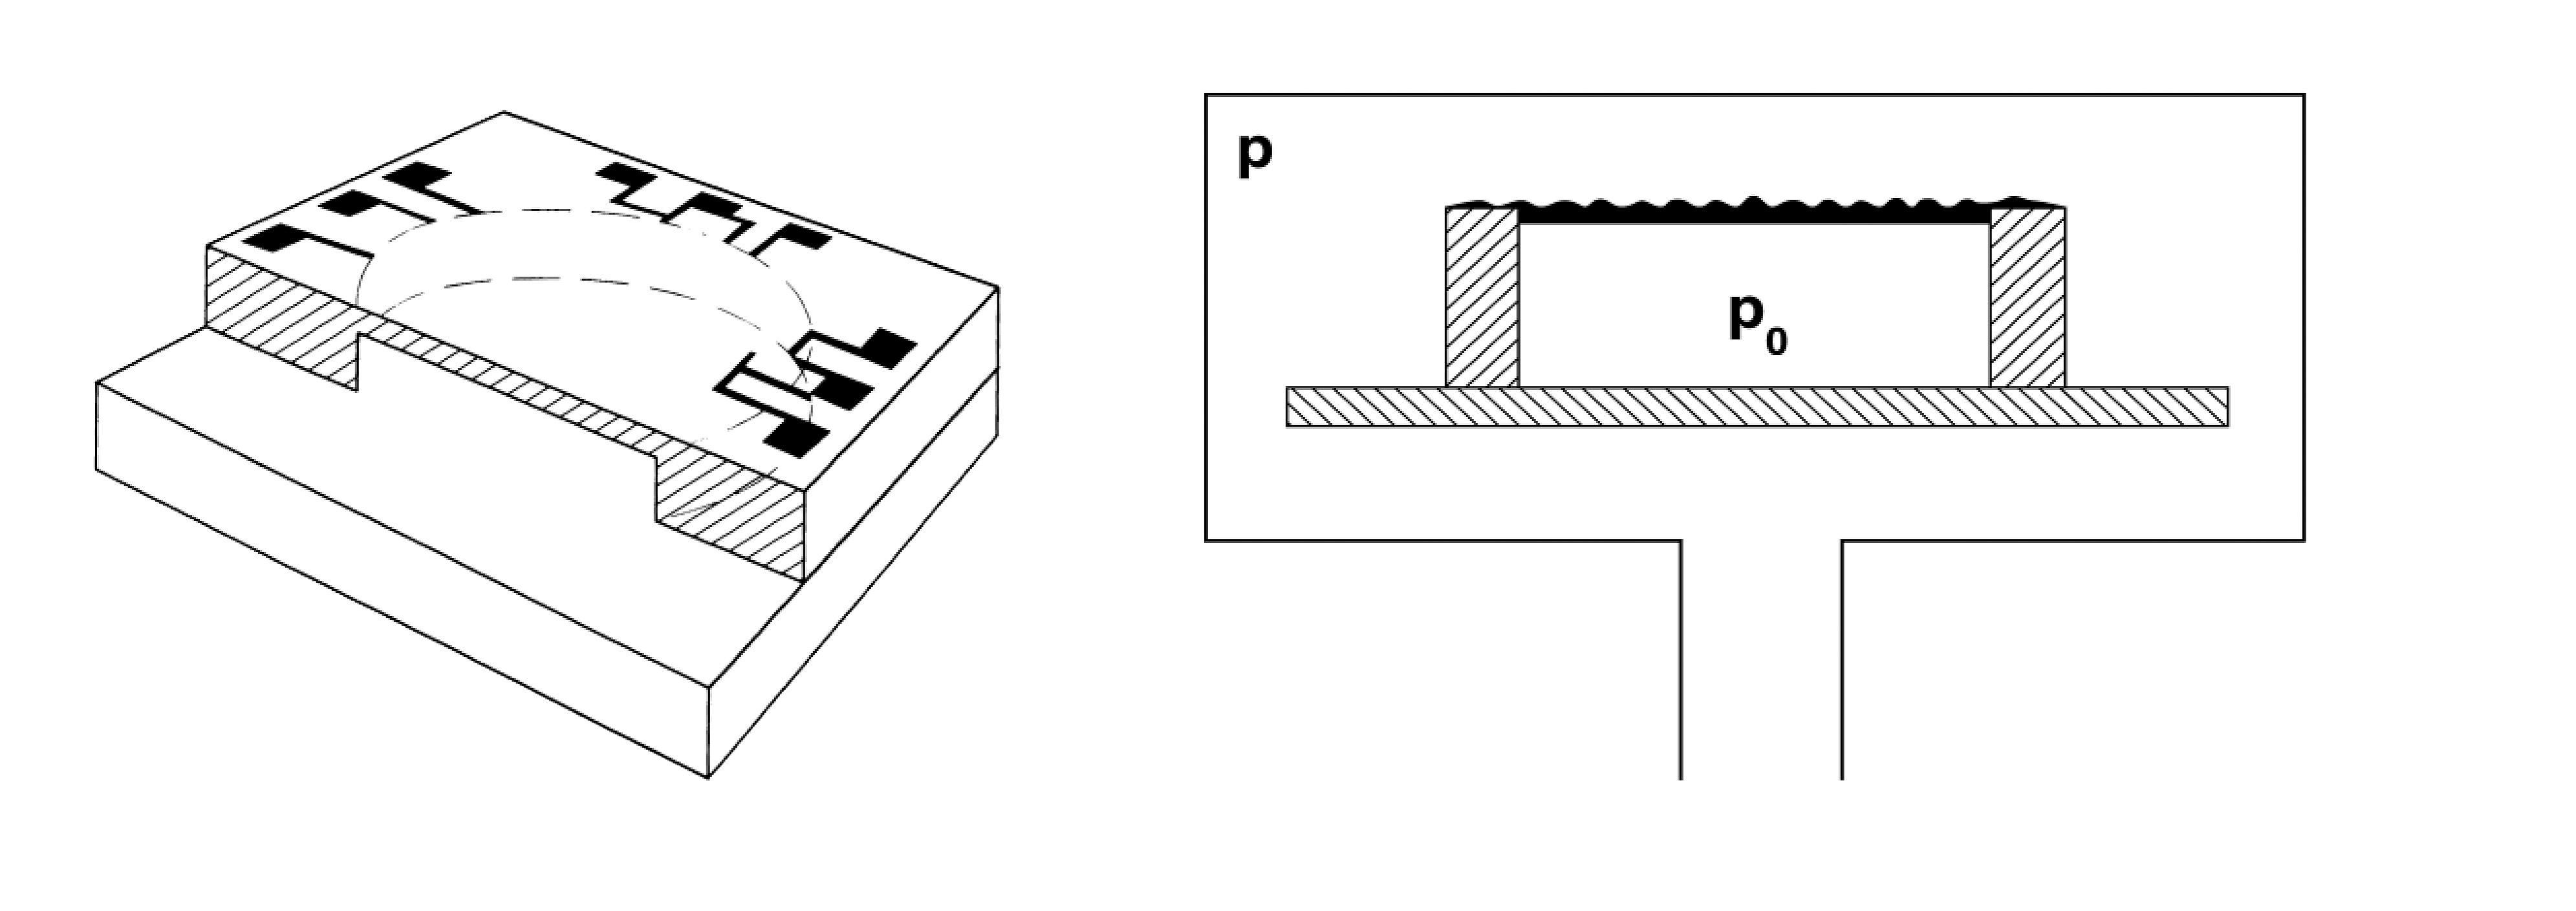
\includegraphics[width=0.7\textwidth]{data/piezo-vakuummeter.jpg}
    \caption{Schematischer Aufbau eines Piezo-Vakuummeters \cite{Druckmessung}.}
    \label{fig:piezo}
\end{figure}


\subsubsection{Pirani-Messröhre}
\label{subsubsec:pirani}

Die Pirani-Messröhre ist ein Druckmessgerät für den Bereich von $\SIrange{10}{e-2}{\hecto\pascal}$. Die Druckmessung beruht auf der linear druckabhängigen Wärmeleitfähigkeit von Gasen in ebendiesem Druckbereich. Aufgrund der Wärmeleitung über die Aufhängung des Drahtes und der Wärmestrahlung ist der Zusammenhang zwischen 
Druck und Wärmeleitfähigkeit jedoch nicht überall linear. Bei Verringerung des Gasdruckes wird weniger Wärme abgeführt, wodurch sich die Temperatur des Drahtes und damit sein Widerstand erhöht. 
Da der Draht an eine Wheatstone'sche Brücke angeschlossen wird, wird ebendiese Differenz im Widerstand gemessen. \newline
Im Bereich von hohen Drücken trägt die Konvektion zum Wärmeaustausch der Gasmoleküle bei, weshalb die Pirani-Messröhre im Bereich eines hohen Druckes nicht funktioniert. In \autoref{fig:pirani} ist die Funktionsweise einer Pirani-Messröhre aufgetragen.

\begin{figure}[H]
    \centering
    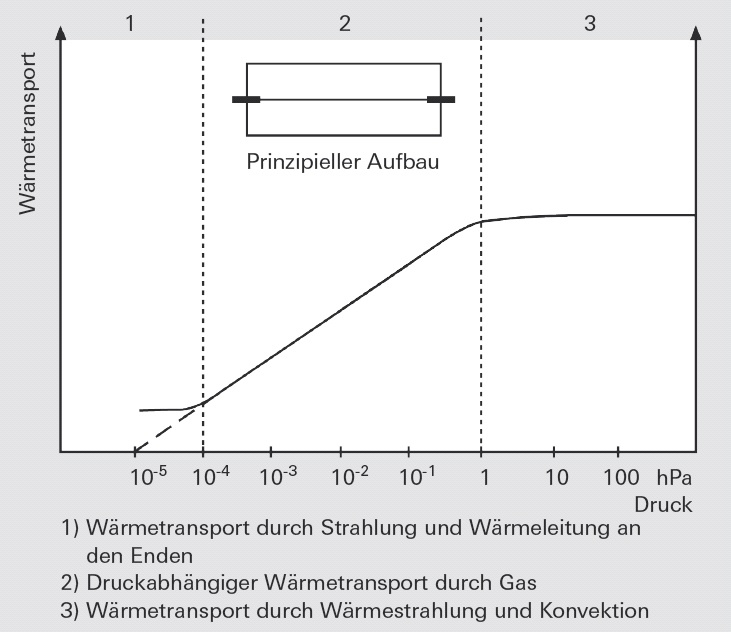
\includegraphics[width=0.7\textwidth]{data/pirani-messroehre.jpg}
    \caption{Funktionsweise einer Pirani Messröhre \cite{Totaldruckmessung}.}
    \label{fig:pirani}
\end{figure}

\subsubsection{Kaltkathoden-Ionisationsvakuummeter}
\label{subsubsec:kaltkathode}

Kaltkathodenvakuumeter bestehen aus einer Anode und einer Kathode, zwischen denen über einen Vorwiderstand eine hohe Spannung angelegt wird. Die Elektronen der Kathode werden durch Feldemission emittiert und auf die Anode beschleunigt.
Dabei ionisieren sie neutrale Gasteilchen, wodurch eine Gasentladung gezündet wird. Dieser Gasentladungsstrom ist ein Maß für den Druck. Da ab $\SI{1}{\hecto\pascal}$ keine Elektronen das Gas ionisieren können,
wird ein invertierbarer Magnetron installiert. Im Inneren der Anode befindet sich nun ein Magnetfeld, durch das sich die Elektronen auf einer Spiralbahn bewegen, wodurch die Wege der Elektronen verlängert und die Stoßwahrscheinlichkeit somit 
erhöht wird. Dadurch werden auch unter $\SI{1}{\hecto\pascal}$ noch genügend Ionen erzeugt. In \autoref{fig:magnetron} ist ein invertierbarer Magnetron nach Hobson und Redhead aufgezeichnet.

\begin{figure}[H]
    \centering
    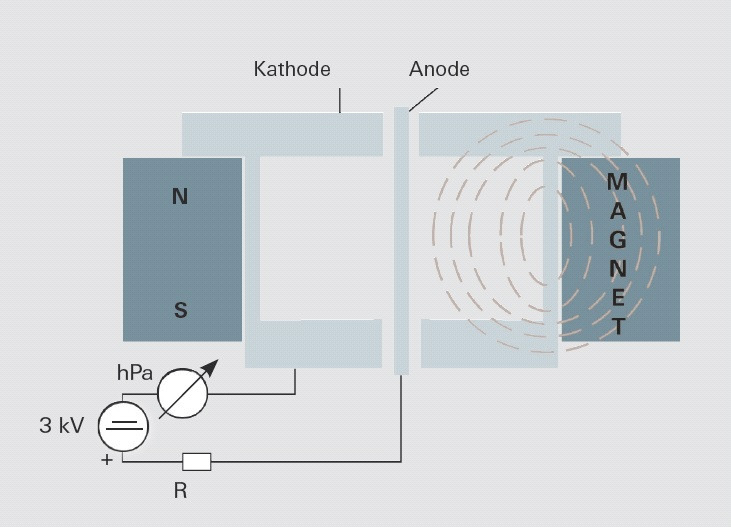
\includegraphics[width=0.7\textwidth]{data/kaltkathode-aufbau.jpg}
    \caption{Aufbau eines invertierten Magnetrons \cite{Totaldruckmessung}.}
    \label{fig:magnetron}
\end{figure}

\subsubsection{Heißkathoden-Ionisationsvakuummeter}
\label{subsubsec:heißkathode}

Im Gegensatz zu Kaltkathodenvakuumeter werden bei Heißkathodenvakuumeter die Elektronen mithilfe einer beheizten Kathode über den glühelektrischen Effekt erzeugt.
In der Mitte einer zylindrischen, gitterförmigen Anode ist ein dünner Draht, der die Ionen auffängt. Genau wie bei dem Kaltkathodenvakuumeter werden durch Elektronenstöße Gasmoleküle ionsiert, wodurch 
Drücke mit hoher Genauigkeit von bis zu $\SI{e-10}{\hecto\pascal}$ gemessen werden können. \autoref{fig:bayardalpertmessroehre} zeigt den Aufbau einer Messröhre nach Bayard-Alpert.

\begin{figure}[H]
    \centering
    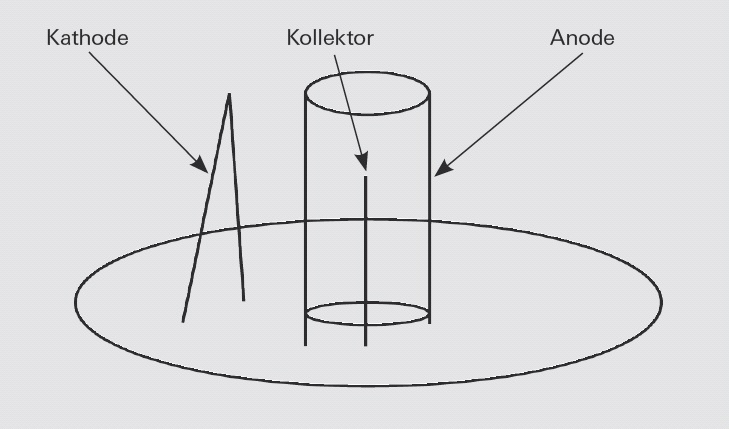
\includegraphics[width=0.7\textwidth]{data/bayard-alpert-messroehre.jpg}
    \caption{Aufbau einer Bayard-Alpert Messröhre \cite{Totaldruckmessung}.}
    \label{fig:bayardalpertmessroehre}
\end{figure}